\documentclass[a5paper]{article}
\usepackage[a5paper, top=8mm, bottom=8mm, left=8mm, right=8mm]{geometry}

\usepackage{polyglossia}
\setdefaultlanguage[babelshorthands=true]{russian}

\usepackage{fontspec}
\setmainfont{FreeSerif}
\newfontfamily{\russianfonttt}[Scale=0.7]{DejaVuSansMono}

\usepackage[font=scriptsize]{caption}

\usepackage{amsmath}
\usepackage{amssymb,amsfonts,textcomp}
\usepackage{color}
\usepackage{array}
\usepackage{hhline}
\usepackage{cite}

\usepackage[hang,multiple]{footmisc}
\renewcommand{\footnotelayout}{\raggedright}

\PassOptionsToPackage{hyphens}{url}\usepackage[xetex,linktocpage=true,plainpages=false,pdfpagelabels=false]{hyperref}
\hypersetup{colorlinks=true, linkcolor=blue, citecolor=blue, filecolor=blue, urlcolor=blue, pdftitle=1, pdfauthor=, pdfsubject=, pdfkeywords=}

\usepackage{tabu}

\usepackage{graphicx}
\usepackage{indentfirst}
\usepackage{multirow}
\usepackage{subfig}
\usepackage{footnote}
\usepackage{minted}

\sloppy
\pagestyle{plain}

\title{Работа с сетью, низкий уровень}
\author{Юрий Литвинов\\\small{yurii.litvinov@gmail.com}}

\date{21.09.2018}

\begin{document}

\maketitle
\thispagestyle{empty}

\section{Архитектура сетей}

Рассказ про сетевое программирование, наверное, стоило бы начать сразу с того, как данные по сети передавать, но в университетском курсе, как мне кажется, должно быть более фундаментальное образование, так что начнём с самого начала. Подробнее про то, как устроены сети, вам ещё расскажут на специально посвящённых этому курсах, у нас будет всего пара занятий про это, но понимать, что происходит, необходимо, чтобы работа с сетью не казалась магией. Понимать, к несчастью, приходится много чего, потому что ``под капотом'' сеть устроена довольно хитро, поэтому сейчас может показаться, что материала очень много и сразу, но делать нечего. Постараюсь особо в подробности не вдаваться. За гораздо более плавным и подробным введением отправлю к классической книге Э. Таненбаум, Д.Уэзеролл. ``Компьютерные сети'' (откуда, кстати, будут позаимствованы многие изображения дальше).

Зачем нужны компьютерные сети и зачем их нужно обязательно уметь программировать, я думаю, объяснять людям, родившимся в 21 веке, уже не надо. Так что начнём сразу с того, как всё устроено. Вот картинка из книжки Таненбаума с общей архитектурой сети Интернет:
\begin{center}
	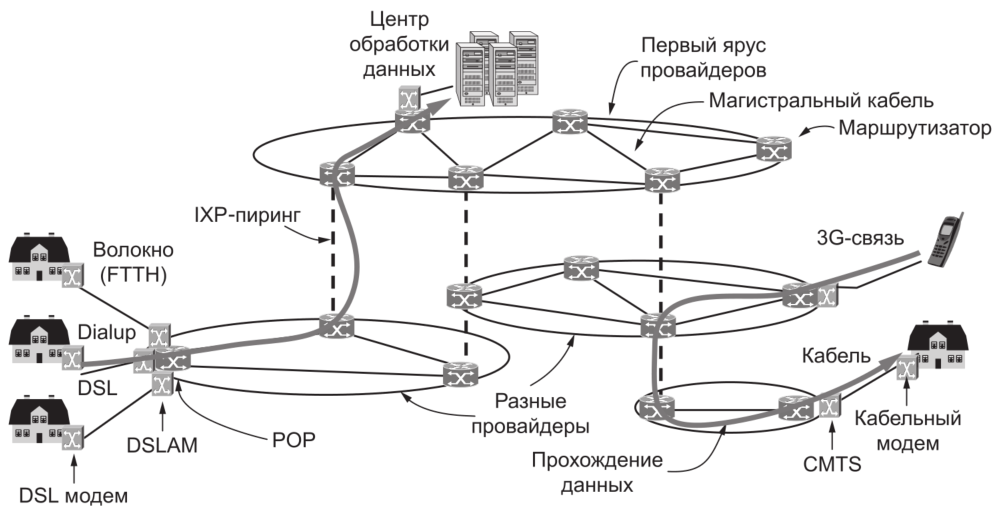
\includegraphics[width=0.9\textwidth]{internetArchitecture.png}
\end{center}

Интернет --- это не единая сеть, а множество сетей разных провайдеров, соединённых в одну так, чтобы отовсюду из сети было доступно всё, что в этой сети находится. Как это работает: есть разные провайдеры, каждый из которых строит свою сеть, чаще всего, непосредственно до потребителей услуг (то есть обычных людей или организаций). При этом для подключения каждого абонента могут использоваться разные технологии. Сейчас это чаще всего Ethernet, бывают оптоволоконные линии, немного устарели, но иногда ещё встречаются DSL-модемы, и, разумеется, разные сорта радиоканалов --- обычный 3G через сеть мобильного оператора, LTE, WiMax. Суть в том, что так или иначе сеть позволяет абоненту общаться с оборудованием провайдера. В случае с Ethernet это обычно маршрутизатор, который стоит в электрощите на лестничной клетке, к нему подключаются все близлежащие абоненты, а из него выходит провод, идущий к следующему маршрутизатору провайдера. Провайдер, в свою очередь, каким бы большим и крутым ни был, не подключён непосредственно ``к интернету'' (просто потому, что такого понятия не существует), а пользуется услугами другого провайдера, и так далее до провайдеров самого высокого уровня, владеющих магистральными линиями, типа трансатлантических подводных кабелей или спутников. Провайдеры также могут соединяться с подсетями соседних провайдеров, чтобы совместно обрабатывать трафик, в этом случае бывает так, что никто никому не платит, а сети используются совместно. Соединение подсетей провайдеров происходит через Internet Exchange Point (IXP), которые представляют собой либо стойку с маршрутизаторами, либо целый датацентр, через который течёт трафик из одной подсети в другую. Есть ряд известных крупных IXP магистральных провайдеров, если одновременно взорвать несколько из них, Интернету станет очень плохо. 

Сложилась такая архитектура по историческим причинам, интернет никто не проектировал, началось всё с ARPANET в США (аж в 1969 году), в Европе примерно в те же времена начали перенимать заокеанский опыт, потом сети объединились (потому что полезность сети зависит квадратично от числа её пользователей, поэтому для любой сети естественно с кем-нибудь объединяться) и получился, собственно, Интернет с мемами, вконтактиком и кучей спама. Изначально сеть создавалась для упрощения совместной работы учёных и правительственных организаций и использовалась в основном для электронной почты.



\end{document}
